% !TEX TS-program = pdflatex
% !TEX encoding = UTF-8 Unicode

% This is a simple template for a LaTeX document using the "article" class.
% See "book", "report", "letter" for other types of document.

\documentclass[11pt]{scrreprt} % use larger type; default would be 10pt

\usepackage[utf8]{inputenc} % set input encoding (not needed with XeLaTeX)
\usepackage{german}
%%% Examples of Article customizations
% These packages are optional, depending whether you want the features they provide.
% See the LaTeX Companion or other references for full information.

%%% PAGE DIMENSIONS
\usepackage{geometry} % to change the page dimensions
\geometry{a4paper} % or letterpaper (US) or a5paper or....
% \geometry{margins=2in} % for example, change the margins to 2 inches all round
% \geometry{landscape} % set up the page for landscape
%   read geometry.pdf for detailed page layout information

\usepackage{graphicx} % support the \includegraphics command and options

% \usepackage[parfill]{parskip} % Activate to begin paragraphs with an empty line rather than an indent

%%% PACKAGES
\usepackage{booktabs} % for much better looking tables
\usepackage{array} % for better arrays (eg matrices) in maths
\usepackage{paralist} % very flexible & customisable lists (eg. enumerate/itemize, etc.)
\usepackage{verbatim} % adds environment for commenting out blocks of text & for better verbatim
\usepackage{subfig} % make it possible to include more than one captioned figure/table in a single float
\usepackage{german}
\usepackage{url}
\usepackage{hyperref}
\usepackage{amsfonts}
\usepackage{amsmath}
\usepackage{amsthm}
\usepackage{listings}
% These packages are all incorporated in the memoir class to one degree or another...

\usepackage{listings}
\usepackage{color}
\definecolor{lightgray}{rgb}{.9,.9,.9}
\definecolor{darkgray}{rgb}{.4,.4,.4}
\definecolor{purple}{rgb}{0.65, 0.12, 0.82}

\lstset{
   language=C++,
   backgroundcolor=\color{lightgray},
   extendedchars=true,
   basicstyle=\footnotesize\ttfamily,
   showstringspaces=false,
   showspaces=false,
   %numbers=left,
   numberstyle=\footnotesize,
   numbersep=9pt,
   tabsize=2,
   breaklines=true,
   showtabs=false,
   captionpos=b
}

%%% HEADERS & FOOTERS
\usepackage{fancyhdr} % This should be set AFTER setting up the page geometry
\pagestyle{fancy} % options: empty , plain , fancy
\renewcommand{\headrulewidth}{0pt} % customise the layout...
\lhead{}\chead{}\rhead{}
\lfoot{}\cfoot{\thepage}\rfoot{}

%%% SECTION TITLE APPEARANCE
\usepackage{sectsty}
\allsectionsfont{\sffamily\mdseries\upshape} % (See the fntguide.pdf for font help)
% (This matches ConTeXt defaults)

%%% ToC (table of contents) APPEARANCE
\usepackage[nottoc,notlof,notlot]{tocbibind} % Put the bibliography in the ToC
\usepackage[titles,subfigure]{tocloft} % Alter the style of the Table of Contents
\renewcommand{\cftsecfont}{\rmfamily\mdseries\upshape}
\renewcommand{\cftsecpagefont}{\rmfamily\mdseries\upshape} % No bold!

%%% END Article customizations

%%% The "real" document content comes below...

\theoremstyle{definition}
\newtheorem*{beisp}{Beispiel}
\newtheorem{definition}{Definition}
\newtheorem*{bemerkung}{Bemerkung}

\title{Paralleles Lesen und Schreiben von farbigen 2D-Barcodes mit MPI}
\subtitle{Seminar Wissenschaftliches Rechnen \\ ZHAW, Zürich}
\author{Florian Lüthi\footnote{\url{luethifl@students.zhaw.ch}}}
%\date{ZHAW (Zürich), 5. Juni 2013} % Activate to display a given date or no date (if empty),
         % otherwise the current date is printed 

\begin{document}
\maketitle

\tableofcontents

\chapter{Einleitung}

Diese Arbeit beschäftigt sich mit der von Md. Mashud Rana, M. E. Kawsar, M. E. Rabbani, S. M. M. Rashid und K. E. U. Ahmed vorgeschlagenen Methode des Lesens und Schreibens von farbigen zweidimensionalen Barcodes mit hoher Datenkapazität \cite{paper}.

Sie beschreibt diese Methode, zeigt eine mögliche Umsetzung des Verfahrens in {\tt C++} mit Parallelisierung mittels {\tt MPI}, und macht eine quantitative Analyse der Implementation in Bezug auf die Performance. Zu guter Letzt zieht sie ein Fazit und überlegt sich den Sinn der angewandten Methode.

Zur Arbeit gehören dieses Dokument sowie die Beispielimplementation. Beides kann von \url{https://github.com/foyan/ColorizedBarCodec} bezogen werden.

Der Autor bedankt sich bei Dr. Alexander Herrigel für die Durchführung des Seminars.

\chapter{Einführung in das Thema}

\section{Existierende Technologien}

Seit den 1970er-Jahren \cite{wiki:barcode} sind Barcodes aus Logistikbetrieben, Supermärkten etc. nicht mehr wegzudenken. Sie bilden das Rückgrat der automatisierten Warenbewirtschaftung. Das Scanning von eindimensionalen Barcodes wie in Abbildung \ref{fig:onedbarcode} ist milliardenfach erprobt und in der Entwicklung eigentlich abgeschlossen.

\begin{figure}
\label{fig:onedbarcode}
\caption{Eindimensionaler Barcode (Quelle: Wikipedia)}
\begin{center}
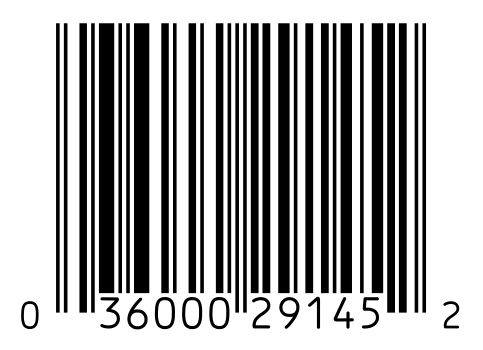
\includegraphics[scale=0.4]{biltli/onedbarcode.png}
\end{center}
\end{figure}

Die Informationsdichte von eindimensionalen Barcodes ist aber sehr beschränkt. Beispielsweise erlaubt die eindimensionale Symbologie UPC-A maximal eine Billion eindeutiger Barcodes \cite{wiki:upc}, was gemäss
\[
\log_2 10^{12} = 39.863\dots
\]
einer maximalen Kapazität von weniger als 5 Bytes entspricht.

Aus diesem Grund wurden mit dem Aufkommen von billigen und sehr akkuraten Kameras in mobilen Devices zweidimensionale Symbologien entwickelt, welche es zumindest erlauben, ganze URLs von Webseiten oder ähnliches zu codieren. Google beispielsweise vermarktet den in Abbildung \ref{fig:qr} ersichtlichen, ursprünglich von Toyota entwickelten {\it Quick Response} Code (QR) \cite{wiki:qr}. Dieser erlaubt es immerhin, maximal 2953 Bytes zu codieren \cite{wiki:qr}.


\begin{figure}
\label{fig:qr}
\caption{QR Code (Quelle: Wikipedia)}
\begin{center}
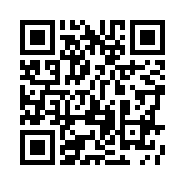
\includegraphics[scale=0.4]{biltli/qr.png}
\end{center}
\end{figure}

Um die Kapazität weiter zu steigern, ist es nötig, eine dritte Dimension einzuführen. Weil aber Hologramme und 3D-Kameras noch nicht marktreif sind, liegt es nahe, die dritte Dimension als Farbe zu codieren. Microsoft geht in seiner Barcode-Technologie {\it High Capacity Color Barcode (HCCB)} seit 2007 \cite{wiki:hccb} genau diesen Weg \cite{ms:hccb}. Ein Beispiel ist in Abbildung \ref{fig:hccb} abgebildet. Die maximale Kapazität von HCCB kann nicht genau genannt werden, weil die Barcodes keine definierte Grösse und Skalierung haben. Labortests scheinen aber gezeigt zu haben, dass es möglich ist, circa 2000 Bytes auf eine Fläche zu codieren, welche nicht viel grösser als eine Ein-Cent-Münze ist. Diese Fläche scheint sich mit einem 600-dpi-Laserdrucker herstellen zu lassen \cite{ms:hccb}.


\begin{figure}
\label{fig:hccb}
\caption{High Capacity Color Barcode (Quelle: Wikipedia)}
\begin{center}
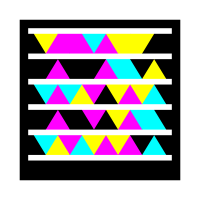
\includegraphics[scale=0.4]{biltli/hccb.png}
\end{center}
\end{figure}

\section{Vorgeschlagene Methode}

\chapter{Randbedingungen}

\chapter{Auswahl der Testdaten für die Arbeit}

\chapter{Algorithmische Beschreibung des Verfahrens}

\chapter{Analyse, Design und Implementierung des Verfahrens}

\chapter{Vergleich der Performancezeiten für ein, zwei oder mehrere CPU-Cores}

\chapter{Zusammenfassung}

\bibliography{biblio}
\bibliographystyle{plain}


\end{document}
